\documentclass[tikz,border=8pt]{standalone}
\usepackage{amsmath,amssymb}
\usetikzlibrary{arrows.meta,automata,positioning,quotes}
\begin{document}
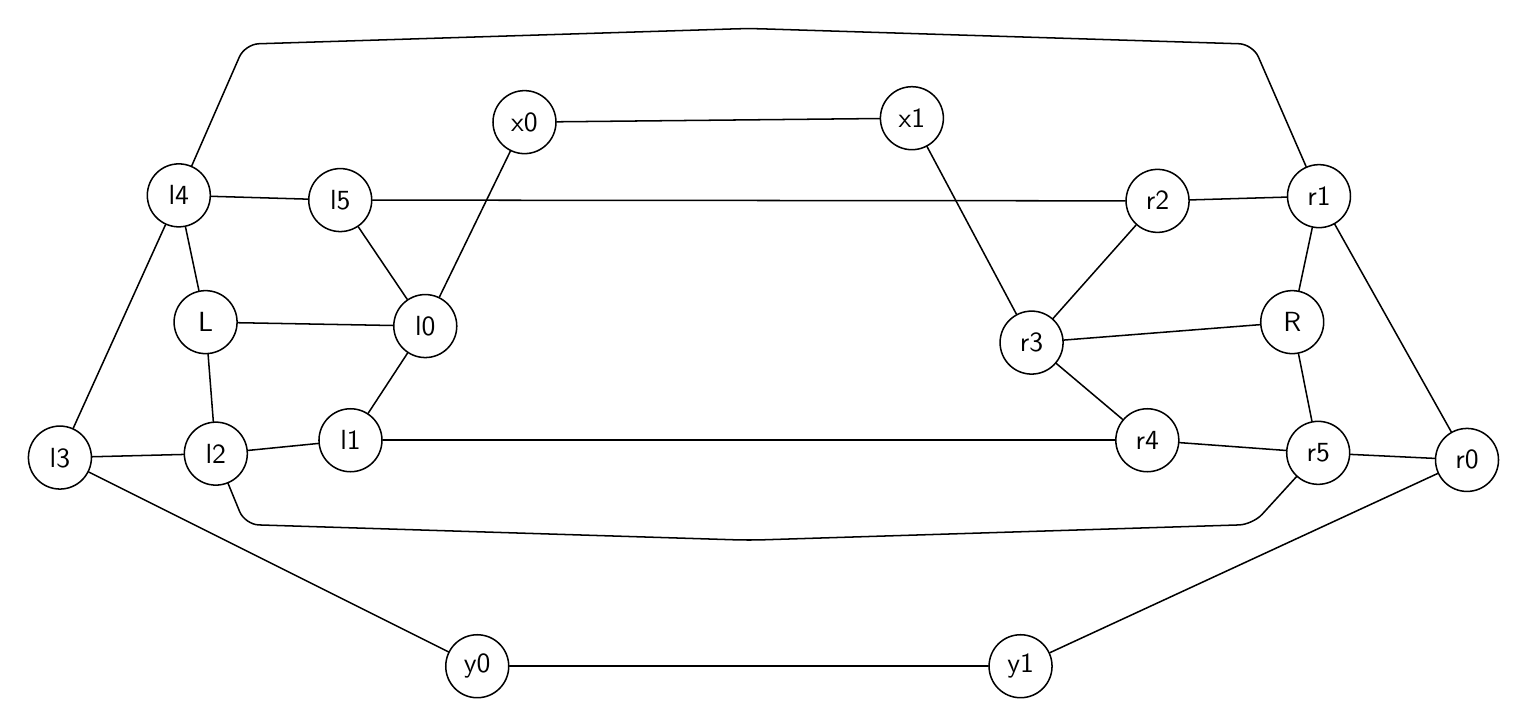
\begin{tikzpicture}[x=1cm,y=1cm]
\tikzset{
  graphnode/.style={circle,draw=black,line width=0.55pt,minimum size=8mm,inner sep=1pt,font=\sffamily},
  graphedge/.style={draw=black,line width=0.55pt,line cap=round,line join=round},
  directed/.style={graphedge,-{Stealth[length=2.4mm,width=2.0mm]}},
  undirected/.style={graphedge}
}
\node[graphnode] (n_L) at (-6.90,0.02) {L};
\node[graphnode] (n_l0) at (-4.11,-0.03) {l0};
\node[graphnode] (n_l1) at (-5.06,-1.48) {l1};
\node[graphnode] (n_l2) at (-6.77,-1.65) {l2};
\node[graphnode] (n_l3) at (-8.75,-1.70) {l3};
\node[graphnode] (n_l4) at (-7.24,1.63) {l4};
\node[graphnode] (n_l5) at (-5.19,1.57) {l5};
\node[graphnode] (n_R) at (6.90,0.02) {R};
\node[graphnode] (n_r0) at (9.12,-1.73) {r0};
\node[graphnode] (n_r1) at (7.24,1.62) {r1};
\node[graphnode] (n_r2) at (5.19,1.56) {r2};
\node[graphnode] (n_r3) at (3.59,-0.24) {r3};
\node[graphnode] (n_r4) at (5.06,-1.48) {r4};
\node[graphnode] (n_r5) at (7.23,-1.64) {r5};
\node[graphnode] (n_x0) at (-2.85,2.56) {x0};
\node[graphnode] (n_x1) at (2.07,2.61) {x1};
\node[graphnode] (n_y0) at (-3.45,-4.35) {y0};
\node[graphnode] (n_y1) at (3.45,-4.35) {y1};
\draw[undirected] (n_l0) -- (n_l1);
\draw[undirected] (n_l1) -- (n_l2);
\draw[undirected] (n_l2) -- (n_l3);
\draw[undirected] (n_l3) -- (n_l4);
\draw[undirected] (n_l4) -- (n_l5);
\draw[undirected] (n_l5) -- (n_l0);
\draw[undirected] (n_L) -- (n_l0);
\draw[undirected] (n_L) -- (n_l2);
\draw[undirected] (n_L) -- (n_l4);
\draw[undirected] (n_r0) -- (n_r1);
\draw[undirected] (n_r1) -- (n_r2);
\draw[undirected] (n_r2) -- (n_r3);
\draw[undirected] (n_r3) -- (n_r4);
\draw[undirected] (n_r4) -- (n_r5);
\draw[undirected] (n_r5) -- (n_r0);
\draw[undirected] (n_R) -- (n_r1);
\draw[undirected] (n_R) -- (n_r3);
\draw[undirected] (n_R) -- (n_r5);
\draw[undirected] (n_l0) -- (n_x0);
\draw[undirected] (n_x0) -- (n_x1);
\draw[undirected] (n_x1) -- (n_r3);
\draw[undirected] (n_l3) -- (n_y0);
\draw[undirected] (n_y0) -- (n_y1);
\draw[undirected] (n_y1) -- (n_r0);
\draw[undirected] (n_l1) -- (n_r4);
\draw[undirected,rounded corners=5pt] (n_l2) -- (-6.40,-2.55) -- (0.00,-2.75) -- (6.40,-2.55) -- (n_r5);
\draw[undirected,rounded corners=5pt] (n_l4) -- (-6.40,3.55) -- (0.00,3.75) -- (6.40,3.55) -- (n_r1);
\draw[undirected] (n_l5) -- (n_r2);
\end{tikzpicture}
\end{document}
